\documentclass[12pt]{beamer}

\usepackage[utf8]{inputenc}
\usepackage{url}
\usepackage{natbib}
\usepackage{textcomp}
\usepackage{graphicx}
\usepackage{booktabs}
\graphicspath{{./img/}}

\usepackage{natbib}
\renewcommand{\bibsection}{\subsubsection*{\bibname } }

\setlength\fboxsep{0pt}
\setlength\fboxrule{0.5pt}

\usetheme{Dresden}

\title{Attacks on wireless localization\\ The case of PKES}
\author{Christian Müller}
\date{4 July 2012}

\section{Introduction}
\subsection*{}
\begin{document}

	\begin{frame}
		\titlepage
	\end{frame}

	\begin{frame}
		\frametitle{Terms}
			\begin{description}
				\item[PKE system]\hfill \\
						\textbf{p}assive \textbf{k}eyless \textbf{e}ntry system
				\item[CID] \hfill \\
					\textbf{C}ustomer \textbf{I}dentification \textbf{D}evice
			\end{description}
	\end{frame}

	\begin{frame}
		\tableofcontents
	\end{frame}
	
\section{Key systems}
\subsection*{}
	\begin{frame}
		\frametitle{Mechanical keys}
		\begin{itemize}
			\item Mechanical key \& lock systems
			\item Immobilisers
		\end{itemize}
	\end{frame}
	
	\begin{frame}
		\frametitle{Remote key Systems}
		\begin{itemize}
			\item Button to open
			\item Operate at RF 	%EU 433 MHz
			\item Physical key to ignite engine
		\end{itemize}
	\end{frame}

	\begin{frame}
		\frametitle{Passive keyless entry systems}
		\begin{itemize}
			\item Car opens when CID is in range
			\item Engine can be ignited if the key is in the vehicle
			\item Physical backup key
		\end{itemize}
	\end{frame}

	\begin{frame}
		\frametitle{PKES in detail}
		\begin{enumerate}
			\item Pulling handle transmits a LF-signal
			\item CID wakes up and responds in RF
			\item If response is correct, the vehicle opens
		\end{enumerate}
		\begin{itemize}
			\item Same holds for ingiting the engine
			\item Usually enhanced by RFID
		\end{itemize}
	\end{frame}

\section{Relay attacks}
\subsection*{}
	\begin{frame}
	\frametitle{Introduction}
		\begin{itemize}
			\item Relocating signal emission \& reception
			\item Underlying problem: proper localization in wireless networks
			\item Circumvents higher level authentication
		\end{itemize}
	\end{frame}

	\begin{frame}
		\frametitle{Two thieves}
		\begin{itemize}
			\item Thief 1 next to the vehicle
			\item Thief 2 near the CID
			\item Relay between both thieves
		\end{itemize}
	\end{frame}
	
	\begin{frame}
	\frametitle{Relay over the cable}
		\begin{center}
			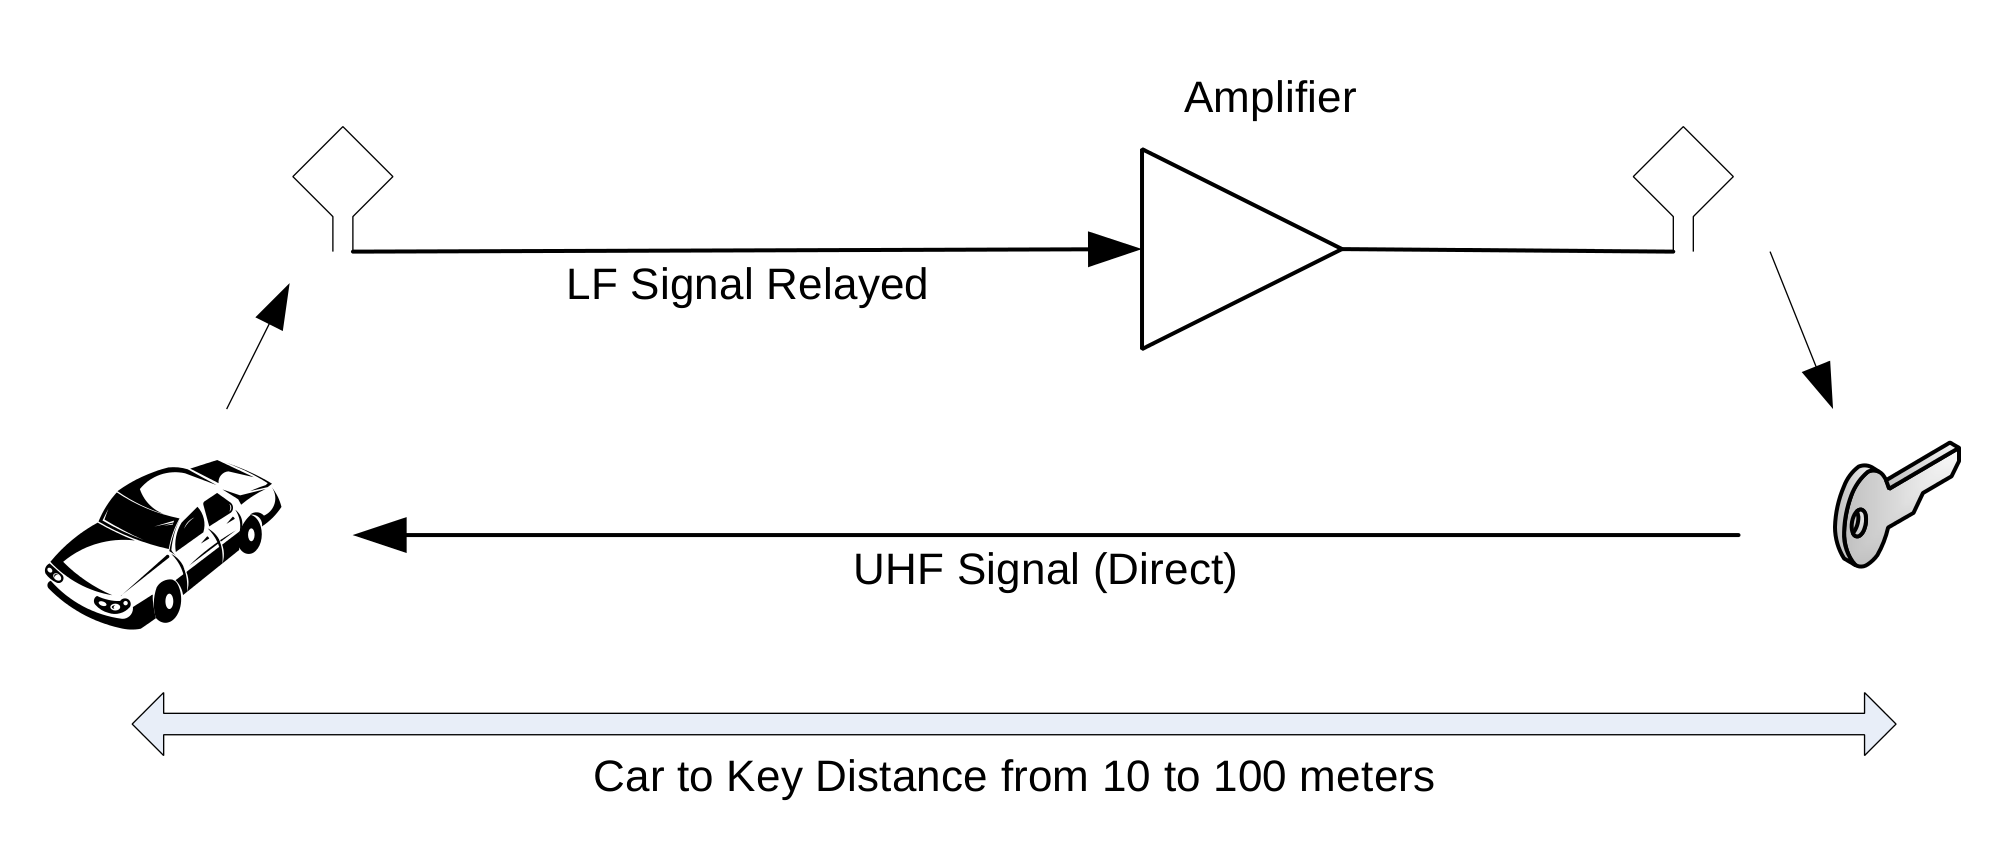
\includegraphics[scale=0.85]{img/franc_relay_over_the_wire.png} 
		\end{center}
	\end{frame}
	
	\begin{frame}
		\frametitle{Relay over the wire}
		\begin{center}
			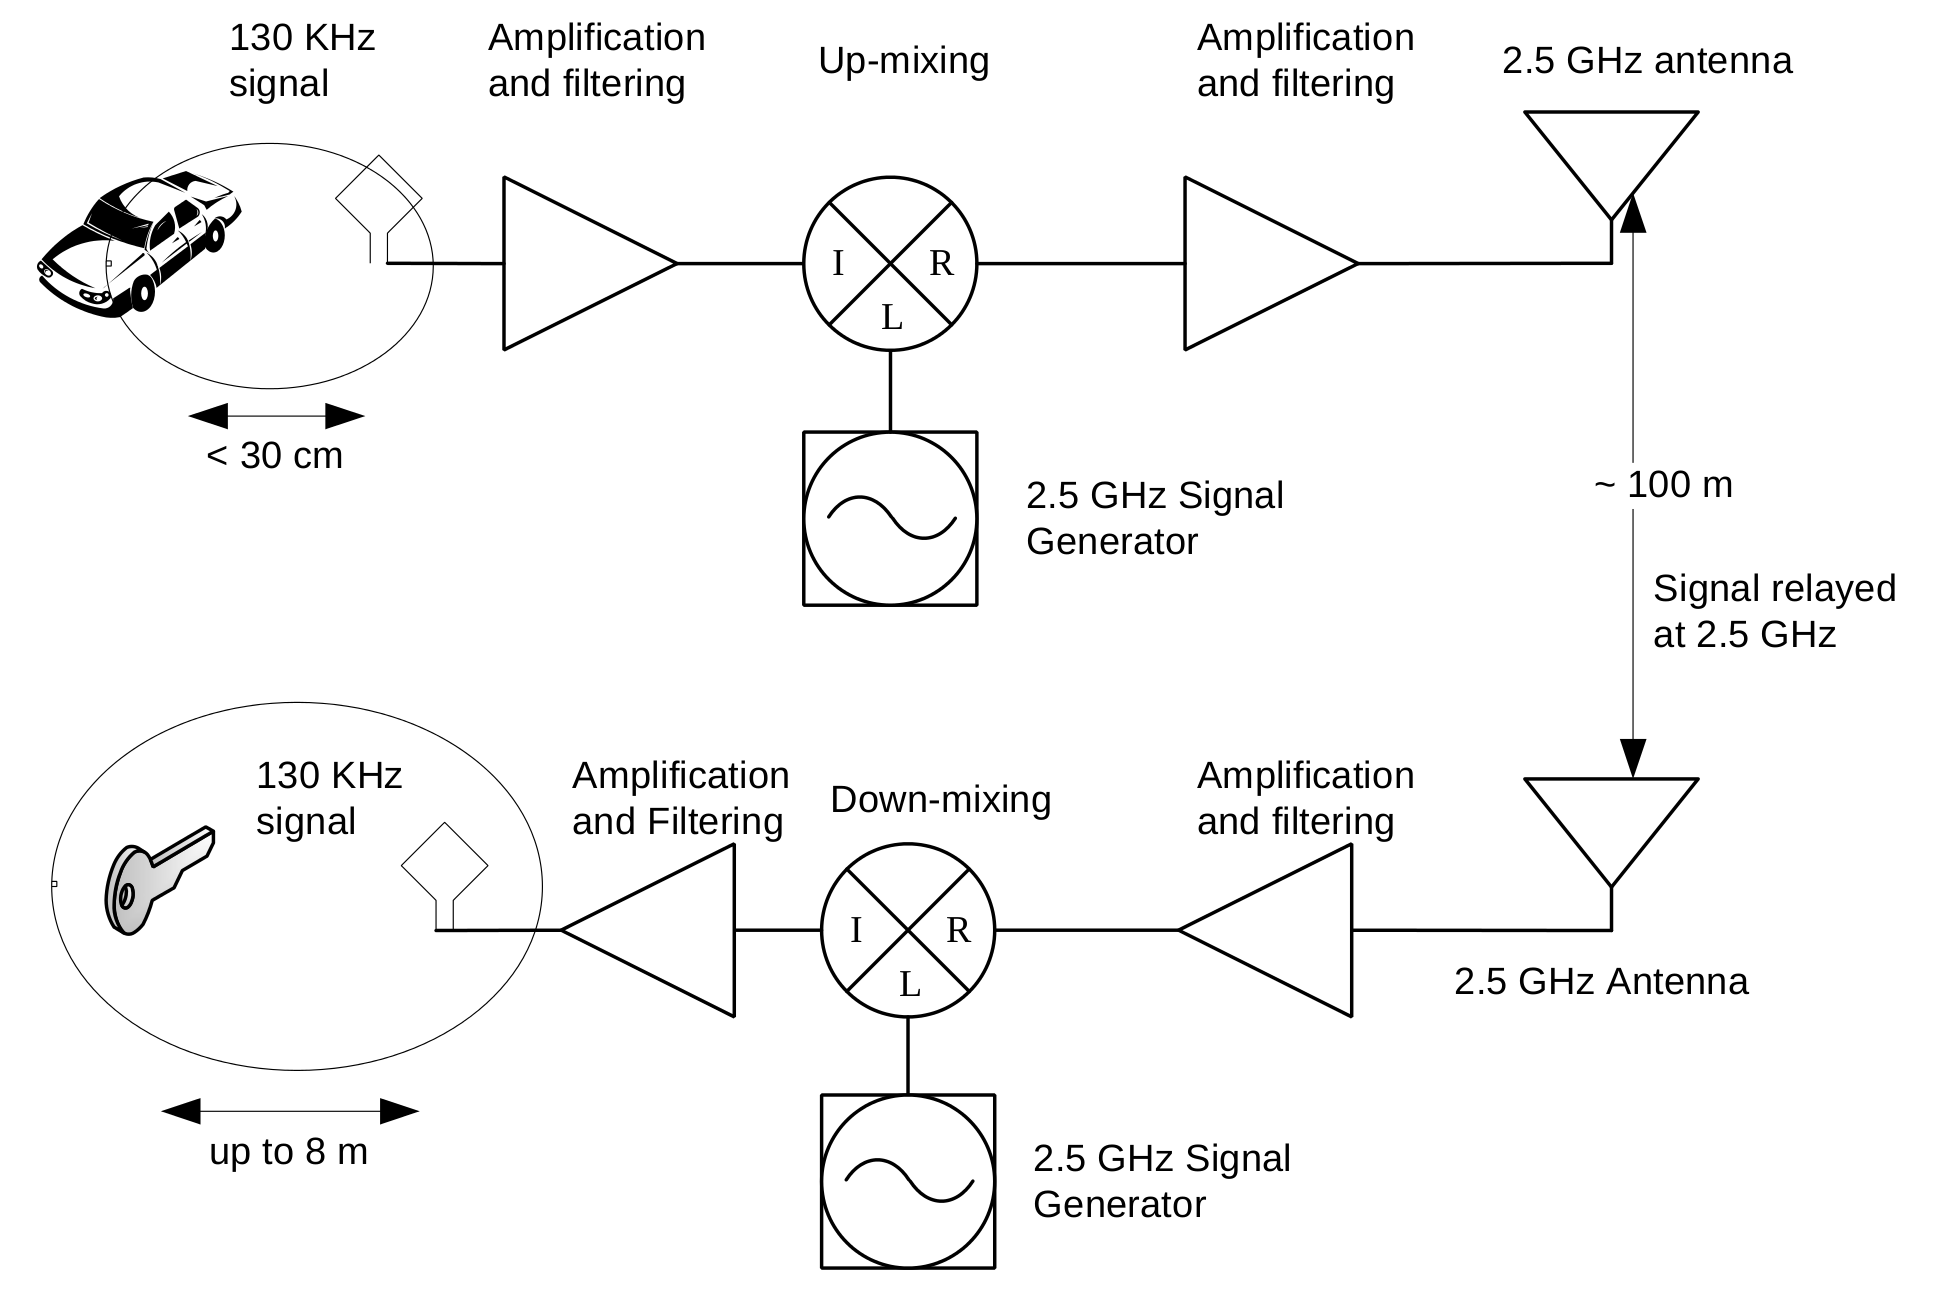
\includegraphics[scale=0.75]{img/franc_relay_over_the_air.png} 	
		\end{center}
	\end{frame}

	\begin{frame}
		\frametitle{This works in practice}
		\begin{itemize}
			\item Simple \& inexpensive
			\item Tested by \citet*{relayAttacksFranc}
			\item All ten systems vulnerable
		\end{itemize}
	\end{frame}

	\begin{frame}
		\frametitle{Results of tests}
		\tiny
		\begin{table}[t]
			\centering
			\begin{tabular}{l r l r l r l}
				\toprule
				Car model	&	\multicolumn{2}{l}{Maximum Delay}	&	\multicolumn{2}{l}{Key Response (std dev)}	&	\multicolumn{2}{l}{Key Response Time Spread}\\
				\midrule
						1 		&	500 			&\textmu s	&	1782  &	\textmu s		(\textpm 8)	&	21		&\textmu s \\
						2 		&	5000			& \textmu s	&	11376 & \textmu s  (\textpm 15)		&	47		&\textmu s \\
						4 		&	500 			&\textmu s	&	-		&										&	- 		&	\\
						5 		&	1000			& \textmu s	&	5002	& \textmu s  	(\textpm 4)		&	11		&\textmu s \\
						6 		&	10000-20000	& \textmu s	&	23582 & \textmu s 	 (\textpm 196)	&	413	&	\textmu s \\
						7 		&	620 			&\textmu s	&	1777	& \textmu s  	(\textpm 12)	&	25		&\textmu s \\
						8 		&	620 			&\textmu s	&	437	& \textmu s  	(\textpm 70)	&	162	&	\textmu s \\
						9 		&	2000			& \textmu s	&	1148	& \textmu s  	(\textpm 243)	&	436	&	\textmu s \\
						10 	&	35 			& \textmu s	&	2177	&\textmu s  	(\textpm 8)		&	12		&\textmu s \\
				\bottomrule
			\end{tabular}
			\caption{Experimentally tested maximum delay, key response time and spread per model, from \cite{relayAttacksFranc}}
			\label{tab:francTimings}
		\end{table}
	\end{frame}

	\begin{frame}
		\frametitle{Results of tests}
		\begin{itemize}
			\item Attack works on all systems
			\item For ``convenient'' attack, amplification is required
			\item Relay can be established over long distances
		\end{itemize}
	\end{frame}

	\begin{frame}
		\frametitle{Scenarios}
		\begin{itemize}
			\item Supermarket
			\item Office
		\end{itemize}
	\end{frame}

	\begin{frame}
		\frametitle{Implications}
			\begin{itemize}
				\item Steal the car
				\onslide<2-2>
				\item Access to the vehicle \\
				\textrightarrow ``Experimental Security Analysis of a Modern Automobile'' by	\citet{expModernAuto}
			\end{itemize}
	\end{frame}

\section{Proposed Solutions}
\subsection*{}
	\begin{frame}
		\frametitle{}
		\begin{description}
			\onslide<1-3>
			\item[short term] \hfill \\
				\begin{itemize}
					\item Fall back to mechanical keys 
				\end{itemize}
			\onslide<2-3>
			\item[long term] \hfill \\
				\begin{itemize}
					\item Highlight action on the CID
				\end{itemize}
			\onslide<3-3>
			\item[long term] \hfill \\
				\begin{itemize}
					\item	Multi channel \citep{multichannelPrevRelay}
					\item Distance bounding protocols \citep{distanceBoundingProtocols}
				\end{itemize}
		\end{description}
	\end{frame}

	\begin{frame}
		\frametitle{Multichannel communication}
			\begin{itemize}
				\item Use two frequencies or types of media
				\item Makes relaying more difficult %TODO because..
				\item More difficult to implement
			\end{itemize}
	\end{frame}

	\begin{frame}
		\frametitle{Distance bounding protocols}
			\begin{itemize}
				\item Be quick
				\item Be strict on timing
				\item Has vulnerabilities
			\end{itemize}
	\end{frame}

	\begin{frame}
		\frametitle{Distance bounding protocol}
			\begin{enumerate}
				\item A generates a nonce
				\item A sends nonce in reverse bitorder to B and starts timer
				\item B will respond with the xored nonce in correct bit order
				\item A stops timer upon receiving of the correctly xored nonce
				\item A deduces distance from time-of-flight
			\end{enumerate}
	\end{frame}

\section{Summary \& Literature}
\subsection*{}
	\begin{frame}
		\frametitle{Summary}
			\begin{itemize}
				\item PKE systems are vulnerable to relay attacks 
				\item Attacks can be performd easily
				\item Solutions are at hand, but not free from vulnerabilities
			\end{itemize}
	\end{frame}
	\begin{frame}
		%TODO fix size
	\frametitle{Literature}
	\tiny
	\nocite{*}
		\def\newblock{}
		\bibliographystyle{plainnat}
		\bibliography{presentation}
	\end{frame}
	
	\begin{frame}
		\begin{center}
			Questions?
		\end{center}
	\end{frame}	

	\begin{frame}
		\frametitle{Thank you!}
		\begin{center}
			Thank you for your attention!
		\end{center}
	\end{frame}	

\end{document}
\end{input}
